\nofiles\documentclass[11pt]{report}
\usepackage[letterpaper, total={6.5in, 10in}]{geometry}

\usepackage{amsmath, amsthm, mathpazo, epic, eepic, color, array}
\usepackage{amssymb}
\usepackage{gensymb}

\usepackage{cancel}
\usepackage{pgfplots}
\usepackage{multicol}
\pgfplotsset{compat=1.13}
\usepackage{etoolbox}
\usepackage{setspace}
\makeatletter
\patchcmd{\chapter}{\if@openright\cleardoublepage\else\clearpage\fi}{}{}{}
\makeatother
\usepackage{hyperref}

\usepackage{enumerate}
%\usepackage{enumitem}
\usepackage[shortlabels]{enumitem}

\usepackage{tikz}
\usetikzlibrary{positioning,chains,fit,shapes,calc,arrows,patterns}
\usepackage{tkz-graph}
\usetikzlibrary{arrows, petri, topaths}
\usepackage{tkz-berge}
\usepackage[all]{xy}
\usepackage{textcomp}

\newlength\tindent
\setlength{\tindent}{\parindent}
\setlength{\parindent}{0pt}
\renewcommand{\indent}{\hspace*{\tindent}}
\newcommand{\ds}{\displaystyle}

\usepackage{lipsum}
\usepackage{pgfplots}
\pgfplotsset{colormap={coloronemap}{rgb=(.4,.4,1); rgb=(.8,.8,1)}}
\pgfplotsset{colormap={colortwomap}{rgb=(1,.4,.4); rgb=(1,.8,.8)}}
%\pgfplotsset{compat=1.3}
\usepackage{eso-pic,calc}
\usepackage[font=small]{caption}
\usepgfplotslibrary{external}
\usetikzlibrary{calc}
\usetikzlibrary{shadings}

\usepackage[h]{esvect}

\pgfplotsset{compat=1.8}

\newboolean{colorprint}
\setboolean{colorprint}{true}
%\setboolean{colorprint}{false}

\ifthenelse{\boolean{colorprint}}{%
\newcommand{\colorone}{blue}
\newcommand{\colortwo}{red}
\newcommand{\coloronefill}{blue!15!white}
\newcommand{\colortwofill}{red!15!white}
\newcommand{\colormapone}{rgb=(.4,.4,1); rgb=(.8,.8,1)}
\newcommand{\colormaptwo}{rgb=(1,.4,.4); rgb=(1,.8,.8)}
\newcommand{\colormapplaneone}{rgb=(.7,.7,1); rgb=(.9,.9,1)}
\definecolor{colormaponebottom}{rgb}{.4,.4,1}
\definecolor{colormaponetop}{rgb}{.8,.8,1}
\definecolor{colormaptwobottom}{rgb}{1,.4,.4}
\definecolor{colormaptwotop}{rgb}{1,.8,.8}
}% ends color
{% not color
\newcommand{\colorone}{black}
\newcommand{\colortwo}{black!50!white}
\newcommand{\coloronefill}{black!15!white}
\newcommand{\colortwofill}{black!05!white}
\newcommand{\colormapone}{rgb=(.4,.4,.4); rgb=(.7,.7,.7)}
\newcommand{\colormaptwo}{rgb=(.6,.6,.6); rgb=(.9,.9,.9)}
\newcommand{\colormapplaneone}{rgb=(.8,.8,.8); rgb=(.95,.95,.95)}
\definecolor{colormaponebottom}{rgb}{.4,.4,.4}
\definecolor{colormaponetop}{rgb}{.7,.7,.7}
\definecolor{colormaptwobottom}{rgb}{.6,.6,.6}
\definecolor{colormaptwotop}{rgb}{.9,.9,.9}
}%
\newcommand{\la}{\left\langle}
\newcommand{\ra}{\right\rangle}
\newcommand{\dotp}[2]{\ensuremath{\vec #1 \cdot \vec #2}}
\newcommand{\proj}[2]{\ensuremath{\text{proj}_{\,\vec #2}{\,\vec #1}}}

\newcommand{\fp}{\ensuremath{f\,'}}

\DeclareMathOperator{\sech}{sech}
\DeclareMathOperator{\csch}{csch}


\pgfplotsset{my style/.append style={axis x line=middle, axis y line=middle, xlabel={$x$}, ylabel={$y$}, axis equal }}

\begin{document}

Section 7.1 Problems to add

Given the graph of $f$, sketch the graph of $f^{-1}$.

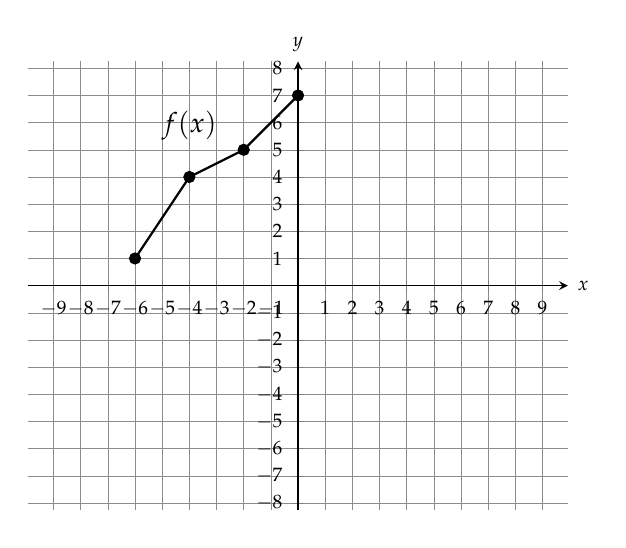
\begin{tikzpicture}  
\begin{axis}[ axis equal,axis x line=middle, axis y line=middle,xmin=-9, xmax=9, ymin=-8.25, ymax=8.25,name=myplot,yticklabel style={{font=\scriptsize}},xticklabel style={{font=\scriptsize}}, xtick={-9,-8,-7,-6,-5,-4,...,5,6,7,8,9}, ytick={-8,-7,-6,-5,-4,...,5,6,7,8},%xticklabel={-8,-7,-6,-5,-4,...,5,6,7,8},
,ymajorgrids=true, xmajorgrids=true, yminorgrids=true, xminorgrids=true,major grid style={line width=.2pt,draw=gray!90}]
\draw[thick] (axis cs:-6,1)--(axis cs:-4,4);
\draw[thick] (axis cs:-4,4)--(axis cs:-2,5);
\draw[thick] (axis cs:-2,5)--(axis cs:0,7);
\addplot[mark=*,only marks] coordinates {(-6,1)(-4,4)(-2,5)(0,7)};

\node[above] at (axis cs:-4,5) {$f(x)$};
\end{axis}
\node [right] at (myplot.right of origin) {\scriptsize $x$};
\node [above] at (myplot.above origin) {\scriptsize $y$};
\end{tikzpicture}

Solution: \\ 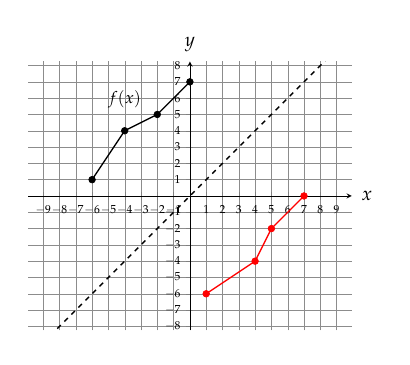
\begin{tikzpicture}  [scale=.6]
\begin{axis}[ axis equal,axis x line=middle, axis y line=middle,xmin=-9, xmax=9, ymin=-8.25, ymax=8.25,name=myplot,yticklabel style={{font=\scriptsize}},xticklabel style={{font=\scriptsize}}, xtick={-9,-8,-7,-6,-5,-4,...,5,6,7,8,9}, ytick={-8,-7,-6,-5,-4,...,5,6,7,8},%xticklabel={-8,-7,-6,-5,-4,...,5,6,7,8},
,ymajorgrids=true, xmajorgrids=true, yminorgrids=true, xminorgrids=true,major grid style={line width=.2pt,draw=gray!90}]
\draw[thick] (axis cs:-6,1)--(axis cs:-4,4);
\draw[thick] (axis cs:-4,4)--(axis cs:-2,5);
\draw[thick] (axis cs:-2,5)--(axis cs:0,7);
\addplot[mark=*,only marks] coordinates {(-6,1)(-4,4)(-2,5)(0,7)};

\draw[thick,red] (axis cs:1,-6)--(axis cs:4,-4);
\draw[thick,red] (axis cs:4,-4)--(axis cs:5,-2);
\draw[thick,red] (axis cs:5,-2)--(axis cs:7,0);
\addplot[mark=*,only marks,red] coordinates {(1,-6)(4,-4)(5,-2)(7,0)};
\addplot[domain=-9:9,black, thick,smooth,dashed] {x};
\node[above] at (axis cs:-4,5) {$f(x)$};
\end{axis}
\node [right] at (myplot.right of origin) {\scriptsize $x$};
\node [above] at (myplot.above origin) {\scriptsize $y$};
\end{tikzpicture}

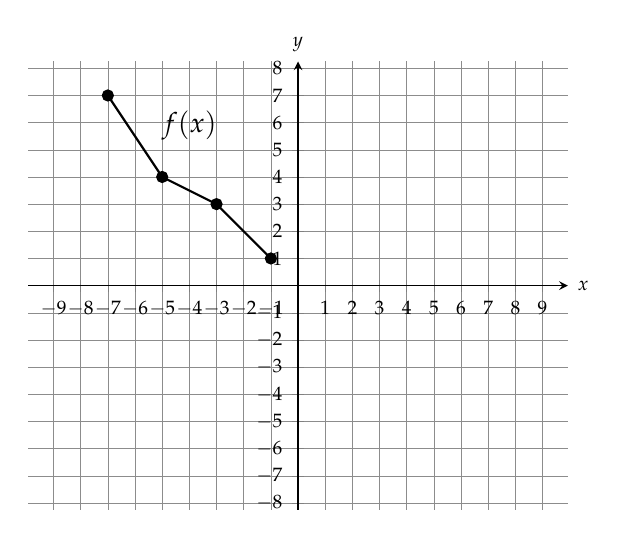
\begin{tikzpicture}  
\begin{axis}[ axis equal,axis x line=middle, axis y line=middle,xmin=-9, xmax=9, ymin=-8.25, ymax=8.25,name=myplot,yticklabel style={{font=\scriptsize}},xticklabel style={{font=\scriptsize}}, xtick={-9,-8,-7,-6,-5,-4,...,5,6,7,8,9}, ytick={-8,-7,-6,-5,-4,...,5,6,7,8},%xticklabel={-8,-7,-6,-5,-4,...,5,6,7,8},
,ymajorgrids=true, xmajorgrids=true, yminorgrids=true, xminorgrids=true,major grid style={line width=.2pt,draw=gray!90}]
\draw[thick] (axis cs:-7,7)--(axis cs:-5,4);
\draw[thick] (axis cs:-5,4)--(axis cs:-3,3);
\draw[thick] (axis cs:-3,3)--(axis cs:-1,1);
\addplot[mark=*,only marks] coordinates {(-7,7)(-5,4)(-3,3)(-1,1)};

\node[above] at (axis cs:-4,5) {$f(x)$};
\end{axis}
\node [right] at (myplot.right of origin) {\scriptsize $x$};
\node [above] at (myplot.above origin) {\scriptsize $y$};
\end{tikzpicture}

Solution: \\
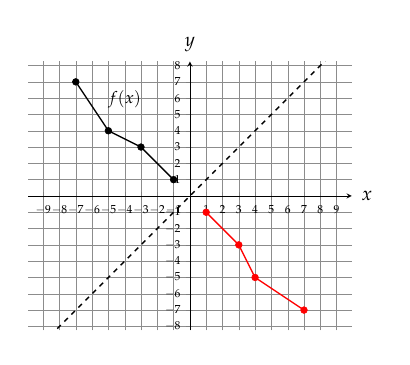
\begin{tikzpicture}  [scale=.6]
\begin{axis}[ axis equal,axis x line=middle, axis y line=middle,xmin=-9, xmax=9, ymin=-8.25, ymax=8.25,name=myplot,yticklabel style={{font=\scriptsize}},xticklabel style={{font=\scriptsize}}, xtick={-9,-8,-7,-6,-5,-4,...,5,6,7,8,9}, ytick={-8,-7,-6,-5,-4,...,5,6,7,8},%xticklabel={-8,-7,-6,-5,-4,...,5,6,7,8},
,ymajorgrids=true, xmajorgrids=true, yminorgrids=true, xminorgrids=true,major grid style={line width=.2pt,draw=gray!90}]
\draw[thick] (axis cs:-7,7)--(axis cs:-5,4);
\draw[thick] (axis cs:-5,4)--(axis cs:-3,3);
\draw[thick] (axis cs:-3,3)--(axis cs:-1,1);
\addplot[mark=*,only marks] coordinates {(-7,7)(-5,4)(-3,3)(-1,1)};

\addplot[domain=-9:9,black, thick,smooth,dashed] {x};
\draw[thick,red] (axis cs:7,-7)--(axis cs:4,-5);
\draw[thick,red] (axis cs:4,-5)--(axis cs:3,-3);
\draw[thick,red] (axis cs:3,-3)--(axis cs:1,-1);
\addplot[mark=*,only marks,red] coordinates {(7,-7)(4,-5)(3,-3)(1,-1)};
\node[above] at (axis cs:-4,5) {$f(x)$};
\end{axis}
\node [right] at (myplot.right of origin) {\scriptsize $x$};
\node [above] at (myplot.above origin) {\scriptsize $y$};
\end{tikzpicture}

Find the inverse of the following functions.

$\ds f(x)=\frac{x+1}{x-2}$ 

$f(x)=x^2 +4$

$f(x)=e^{x+3}-2$

$f(x)=\ln(x-5)+1$

Add to the group 13-18

$\sin^{-1}(-\sqrt3 /2)$   Solution: $-\frac{\pi}{3}$

$\cos^{-1}(-\sqrt2/2)$  Solution: $\frac{3\pi}{4}$

$\cos^{-1}(\cos(8\pi/7))$  Solution: $\frac{6\pi}{7}$

Simplify the following. %%%%%%%%%%%%%%%%% Check the directions here....

$\ds \sin \biggl(\tan^{-1} \frac{x}{\sqrt{x^2-4}}\biggr)$

$\ds \tan \biggl(\sin^{-1} \frac{x}{\sqrt{x^2-4}}\biggr)$

$\ds \cos \biggl(\sin^{-1} \frac{5}{\sqrt{25-x^2}}\biggr)$

$\ds \cot \biggl(\cos^{-1} \frac{3}{\sqrt{x}}\biggr)$



\end{document}